\documentclass[a4paper,12pt,final]{article}
\usepackage{graphicx}
\usepackage{multicol}					
\setlength{\multicolsep}{0pt}
\title{
\begin{center}
  	
\includegraphics[scale=0.3]{101Logo.png} 
  \end{center}
  \textbf{\\}
CSIR - Distributed Application Manager\\
Project Management Document\\
}
\author{101 Solutions}

\begin{document}
\maketitle
\begin{center}
Version 0.5
\end{center}
\textbf{\\}
\textbf{\\}
\textbf{\\}
\textbf{\\}
\textbf{\\}
\textbf{\\}
\begin{center}
\begin{tabular}{|l|l|}
\hline
Francois Germishuizen & 11093618\\
\hline
Jaco Swanepoel & 11016354\\
\hline
Henko van Koesveld & 11009315\\
\hline
\end{tabular}
\end{center}
\thispagestyle{empty}
\newpage
\thispagestyle{empty}
\textbf{\large{Change Log}}
\vspace{6pt}\newline
\begin{tabular}{|l|l|l|}
\hline
Date & Version & Description\\
\hline
12 Sept & Version 0.1 & Document Created\\
\hline
12 Sept & Version 0.2 & Added member profiles\\
\hline
12 Sept & Version 0.3 & Added burndown chart\\
\hline
12 Sept & Version 0.4 & Added issue management content\\
\hline
12 Sept & Version 0.5 & Outstanding tasks / risks\\
\hline
\end{tabular}
\newpage
\tableofcontents
\thispagestyle{empty}
\newpage

\pagenumbering{arabic}
\section{Overview}
\subsection{Background}
The CSIR is actively developing a distributed simulation framework that ties
in with various other real systems and is used to exchange information
between them. The client has a number of configurations of this system
depending on the requirements of the client which can involve various
external applications as well.\\
\textbf{\\}
One of the issues the client has is to quickly distribute the latest build or
configuration files of their software over various computers that are needed
for an experiment. In some cases the same computers may be used for other
experiments which mean each of the computers may need to have various
builds and configuration options.\\
\textbf{\\}
Another issue they experience is the running, stopping and restarting of
the complete simulation. During a simulation it may be determined that
certain configuration options may need to be changed and distributed to the
affected machines, in which case either all or some components will need to
be restarted which can become tedious and time consuming.
\subsection{Business opportunity}
The goal of our project is to develop an application which is able to maintain
various build versions of the simulation framework and distribute these builds
to certain designated machines that may be required for an experiment. The
application will monitor system statistics of the various machines attached
to an experiment and will have the ability to execute applications on those
machines which will have different configuration options.\\
\textbf{\\}
The application will consist of a master and slave component where the
master is used to control the distribution of slaves. From the master one will
be able to start an experiment which will run the relevant applications on all
the necessary machines.




\section{Software development process}
The software development process that we have opted for are an agile based approach by which we are able to continually improve on the current state that the project is in. We strive to always have a working project in version control(Git) to ensure that if we need to show our progress, it is there.
\\
We are following a scrum methodology to ensure that our project stays on track. 
\\
Other reasons for taking agile is the continous change that it allows us to incoroporate. This allows us to change when the client changes the requirement and allows us to more easily adapt to that change.


\section{Member Profiles}
\subsection{Francois Germishuizen}
\begin{center}
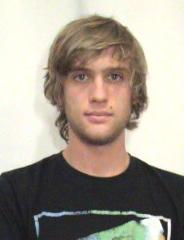
\includegraphics[width=3cm]{Francois.jpg}
\end{center}
\textbf{Skills:}
\begin{itemize}
\item General
\begin{itemize}
\item Web Development
\item Database Design
\item Software Design
\item Particular interest in computer networks
\end{itemize}
\item Programming and Markup Languages
\begin{itemize}
\begin{multicols}{2}
\item C++
	\item C\#
	\item Java
	\item PHP
	\item MySQL
    \item Microsoft SQL Server
	\item XML
    \item XSLT
    \item HTML
    \item CSS
	\item Javascript
    \item Qt, learn't during project
\end{multicols}
\end{itemize}
\end{itemize}
\textbf{Responsibilities:}
\begin{itemize}
\item Continuous work on the main project
\end{itemize}




\subsection{Jaco Swanepoel}
\begin{center}
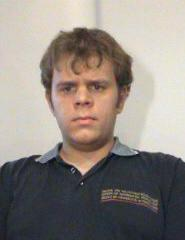
\includegraphics[width=3cm]{jaco.jpg}
\end{center}
\textbf{Skills:}
\begin{itemize}
\item General
\begin{itemize}
\item Organized
	\item Detail Oriented
	\item Reliable
	\item Work well under pressure
\end{itemize}
\item Programming Languages
\begin{itemize}
\begin{multicols}{2}
\item C
    \item C++
	\item C\#
	\item Java
    \item Basic Ruby
    \item Delphi
    \item Qt, learn't during project
\end{multicols}
\end{itemize}
\item Web development
\begin{itemize}
\begin{multicols}{2}
	\item HTML5
	\item CSS3
	\item JavaScript
	\item JSON
    \item JQuery
    \item Microsoft Sql Server
    \item MySql
    \item PHP
    \item XML
    \item Basic XSL
    \item Basic DTD and Schema
\end{multicols}
\end{itemize}
\end{itemize}
\textbf{Responsibilities:}
\begin{itemize}
\item Continuous work on the main project
\item Admin and client communications
\end{itemize}



\subsection{Henko van Koesveld}
\begin{center}
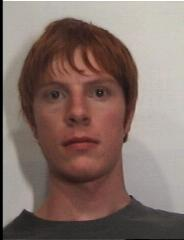
\includegraphics[width=3cm]{Henko.jpeg}
\end{center}
\textbf{Skills:}
\begin{itemize}
\item General
\begin{itemize}
	\item Database Design and Setup as well as normalization
	\item Software design with a focus on extensibility and maintenance
	\item Experience in various programming languages
	\item Hard working, dedicated
	\item Patience in solving problems
	\item Well experienced with HTML5 Web development
	\item Past experience with Qt framework
\end{itemize}
\item Programming and Markup Languages
\begin{itemize}
\begin{multicols}{2}
	\item C++
	\item Qt
	\item C\#
	\item Java
	\item PHP
	\item MySQL, Microsoft SQL Server
	\item XML, XSLT, HTML, CSS, JSON, JQuery, Javascript
	\item Knowledge in Assembly, Ruby and Delphi
\end{multicols}
\end{itemize}
\end{itemize}
\textbf{Responsibilities:}
\begin{itemize}
\item Continuous work on the main project
\item Keep the team updated on some work that needs to be done
\end{itemize}


\newpage
\section{Issue Management}
This section describes how we report issues with the current software as it is and how we will go about resolving those issues. 
\subsection{Priorities}
Each issue is assigned a priority whereby it is handled as such. 
\subsection{Software}
We first opted for a document based bug tracking software. We then later changed bugtracking to an online available form. We have changed to making use of FogBugz which allows us to have a 45 day free period where we can file any.
\\
FogBugz allows us to set certain tasks that are to be done. One can set the priority of the task such as, scale from 4 to 6 for "Fix if time" where one can be able to fix it if there is time, and a scale of 1 to 3 for "Must Fix" where it must be fixed. The last one is 7 which means that it does not have to be fixed.
\\
This website is not however only meant for the use in errors in code, but also things that must be changed and work that needs to be done. Work such as features that is still misssing, or even work that is still to be done. Other features that are used are the dates where we set out dates in which we believe that item should be done and handled.
\\
Our link to the bug tracking and handling site is appman.fogbugz.com. That is where the majority of bug tracking and job tasks are tracked and handled. The goals we set out are prioritized according to how important that is. Thus we can easily see what is more important than other tasks. 

\newpage
\section{Burndown Chart}
\begin{center}
\textbf{Burndown chart as at Friday 6 September, iteration 3 demo\\}
\end{center}
\begin{center}
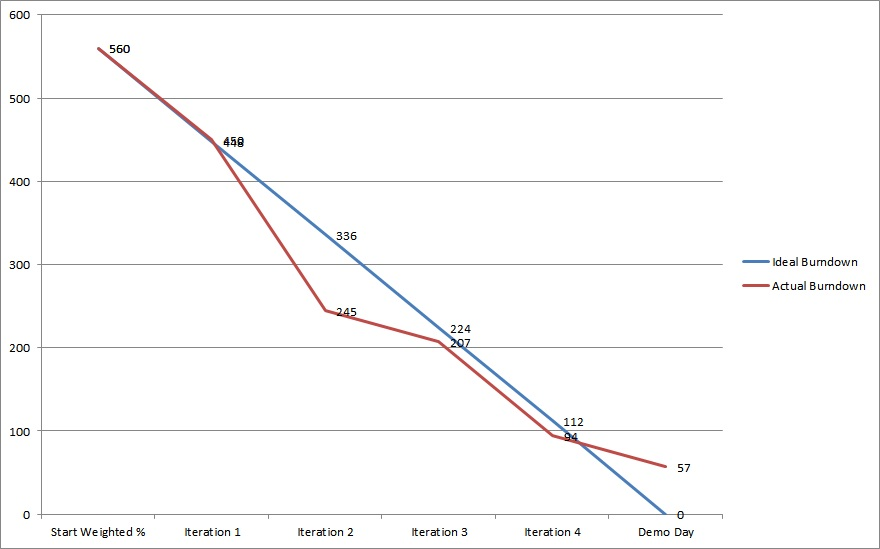
\includegraphics[scale=0.7]{Burndown.jpg}
\end{center}




\section{Outstanding tasks / risks}
We are currently still working on the following things:
\begin{itemize}
\item Simulation creation
\item Simulation execution
\item Storing slave vitals in a MySql database
\item Physical copy of builds
\item Performance issues such as slow md5 generation
\end{itemize}
\end{document}